\documentclass[11pt]{article}
\usepackage{geometry}                % See geometry.pdf to learn the layout options. There are lots.
\geometry{a4paper}
\usepackage{graphicx}
\usepackage{amssymb}
\usepackage{amsmath}
\usepackage{lscape}
\usepackage{multirow}
\usepackage{makeidx}
\usepackage{hyperref}
\usepackage{fancyvrb}

\newcommand{\ciftocell}{\texttt{cif2cell}}

\newenvironment{warning}[1][Warning!]{\begin{trivlist}
\item[\hskip \labelsep {\bfseries #1}]}{\end{trivlist}}
\newcommand{\T}{\rule{0pt}{2.6ex}}
\newcommand{\B}{\rule[-1.2ex]{0pt}{0pt}}
\newcommand{\TM}{\rule{0pt}{6ex}}
\newcommand{\BM}{\rule[-5ex]{0pt}{0pt}}


\title{The \ciftocell{} manual}
\author{Torbj\"orn Bj\"orkman}
%\date{}                                           % Activate to display a given date or no date

\begin{document}
\maketitle
\tableofcontents
\newpage
\section*{Introduction -- Of CIF's and Cells}
An electronic structure program needs atomic positions and, at least in the case of band structure programs, unit cell vectors to calculate the electronic structure of a crystal. Experimental data on the other hand tends to be given as a space group and a set of irreducible, or wyckoff positions, and are often distributed in the form of CIF files. There is a wide range of sources of CIF files --- it is in fact the standard means of communicating crystallographic data for virtually everyone outside of the electronic structure community! Yet far from all electronic structure programs can read the CIF format, and from this circumstance a small set of convenience scripts one day turned into the program \ciftocell.

What the program does is simply to take the crystal structure information in a CIF file, typically space group information and a set of irreducible coordinates, and then set up a calculation cell which is then output to your favourite electronic structure program (ESP). As you are probably aware, the choice of calculation cell for a given crystal is arbitrary and infinitely many possibilities exist for any given crystal. Perhaps the simplest example is when a problem requires us to set up a supercell, which is just describing the same crystal in a different cell than the primitive one, but even the primitive cell can often be chosen in many different ways. \ciftocell{} contains working solutions for choices of primitive cells for (almost) any possible crystal and will make a choice automatically. You may choose either the primitive cell for the given structure, such as the rhombohedral cell with one atom for fcc Cu, or the conventional cell, a cubic cell with four atoms for fcc Cu. These cells can then be used as building blocks for generating supercells by multiplying them up and/or inputting extra vacuum in the structure. 

This manual is intended as a document for computational physicists and materials scientists. The problems that you solve when generating a computational cell from crystallographic data belongs to the field of crystallography and the program is not intended to replace a working knowledge of basic crystallography. Remember this, and refer to your textbook in crystallography or solid state physics/chemistry when you get confused and your life with \ciftocell{} will be happy.

The code was published in \href{http://dx.doi.org/10.1016/j.cpc.2011.01.013}{Computer Physics Communications {\bf 182}, 1183--1186 (2011)}, please cite generously. Happy computing!

\vspace{1.5cm}
Torbj\"orn Bj\"orkman


\newpage
\section{Installation}
\subsection{Requirements}
\ciftocell{} requires Python 2.4 or higher and the PyCIFRW python package\footnote{Available from \texttt{http://pycifrw.berlios.de}.}. Note however that the output may be slightly different (but equivalent) with Python 2.4 than with later versions due to differences in the internal sorting routines of different Python distributions.

To install the program in your systems standard location, type:
\begin{verbatim}
python setup.py install 
\end{verbatim}
To choose a different location, add 
\begin{verbatim}
--prefix=where/you/want/it 
\end{verbatim}
to the above line. For help and more options type
\begin{verbatim}
python setup.py --help
\end{verbatim}


\section{Getting started}

This section is meant to give you a quick overview of how you generate cells to get you started as quickly as possible. Running \ciftocell{} is quick, so the best way to learning to work with it is to simply run it over and over, testing different settings and options until you have what you want. The program comes with a small set of sample CIF files which can be found either in the source distribution or in the directory \texttt{[prefix]/lib/cif2cell/sample\_cifs}, where \texttt{[prefix]} is the path where you installed \ciftocell. The examples below assume that you stand in a directory containing these sample files. In the following, some arbitrary command line input will be specified within brackets \texttt{[like this]}. You are encouraged to run the tests and play around as you read.

\subsection{Help!}
The quickest way to get help in \ciftocell{} is to type
\begin{verbatim}
cif2cell -h
\end{verbatim}
This will list all available input options along with a description.

\subsection{The first run}\label{firstrun}
There is only one required piece of input, and that is the CIF file itself which is given either as an argument to the program:
\begin{verbatim}
cif2cell [someoptions] Si.cif [otheroptions]
\end{verbatim}
and if no output program is specified, the cell information is output to screen:

\begin{verbatim}
CIF2CELL 0.4.0
2011-03-25 16:35
Output for Si (Silicon)
CIF file exported from Inorganic Crystal Structure Database.
Database reference code: 51688.

 BIBLIOGRAPHIC INFORMATION
Toebbens, D.M. et al., Materials Science Forum 378, 288-293 (2001) 

 SYMMETRY INFORMATION
Cubic crystal system.
Space group number     : 227
Hall symbol            : F 4d 2 3 -1d
Hermann-Mauguin symbol : Fd-3mS

 INPUT CELL INFORMATION
Lattice parameters:
          a           b           c 
  5.4305300   5.4305300   5.4305300 
      alpha        beta       gamma 
 90.0000000  90.0000000  90.0000000 
Representative sites :
Atom           a1          a2          a3 
Si      0.0000000   0.0000000   0.0000000

 OUTPUT CELL INFORMATION
Bravais lattice vectors :
  0.5000000   0.5000000   0.0000000 
  0.5000000   0.0000000   0.5000000 
  0.0000000   0.5000000   0.5000000 
All sites, (lattice coordinates):
Atom           a1          a2          a3 
Si      0.0000000   0.0000000   0.0000000
Si      0.2500000   0.2500000   0.2500000
\end{verbatim}

\newpage
First there is some information about the program itself and a description of the compound derived from information in the CIF file. If the file comes from a databases known to \ciftocell, information about that is also printed. Then follows any bibliographic information found in the file. Then starts the actual crystal information with data about the space group. If the \texttt{-v} or \texttt{--print-symmetry-operations} flags are given, all symmetry operations will also be printed here. Next comes the lattice parameters and representative sites (occupied wyckoff positions), with the the chemical elements and, in case of an alloy, another column with the site occupancies. Then follows the things we actually want -- the Bravais lattice vectors and all positions of the atoms.  In the case of Si in the diamond structure the result is probably familiar:  the standard fcc lattice vectors and two atoms in the basis, one at $(0,0,0)$ and another in $(\frac{1}{4},\frac{1}{4},\frac{1}{4})$. 

Having generated the basic cell we want to export that to our favourite ESP. This is done by simply giving the option \texttt{-p espname} or \texttt{--program=espname}. The possible choices for \texttt{espname} can be found in Table \ref{esptable}, where you also find what files will be generated. Let's try this out for someones favourite program VASP. Adding the option \texttt{-p vasp} you will get the above output, properly formatted, to a file called POSCAR:
\begin{verbatim}
Generated by cif2cell 0.4.6 from [...] Species order: Si 
   5.430530
  0.500000000000000   0.500000000000000   0.000000000000000
  0.500000000000000   0.000000000000000   0.500000000000000
  0.000000000000000   0.500000000000000   0.500000000000000
   2
Direct
  0.000000000000000   0.000000000000000   0.000000000000000 
  0.250000000000000   0.250000000000000   0.250000000000000 
\end{verbatim}
Notice that the very long first line containing a lot of information about where the data came from is shortened here (marked by \texttt{[...]}). The important thing to see is that we get a correct output file, and that \ciftocell{} helps you keep track of where the data came from, to the extent that this can be inferred from the CIF file. The last bit of the line,  "Species order: Si", is important. It tells you which the atomic species are that are part of the file, since, in the particular case of VASP, this information is not given here, but in a different file, POTCAR, which was not generated by \ciftocell{}. To enable the user to set up the POTCAR file properly, \ciftocell{} stored the information needed here, but other ways of handling this information are also available, study the ESP specific output options to find out how.


\section{Getting further}
Here we go on discussing more cell generation options and some technical aspects of the cell generation.

\subsection{Cell generation}
By default, \ciftocell{} will reduce the cell to the primitive cell, anticipating that the user wants to calculate something as small as possible, but we can also get the conventional cell. The diamond structure is a cubic system, and the primitive cell has only two atoms. Now try to also give the program the option \texttt{--no-reduce}. You should now get 8 atoms and cubic lattice vectors. Note that the conventional and primitive cell are the same in many systems.\footnote{In all systems which has a space group, or Hermann-Mauguin (H-M), symbol that starts with ''P'' (for ''primitive''). See the example for fcc Si above, where the H-M symbol is 'F', (from German ''Fl\"achenzentriert'', meaning face-centered).}
For the fcc lattice the choice of primitive lattice vectors is straightforward, but in many systems of lower symmetry, in particular monoclinic systems, the choice is not always as simple. \ciftocell{} has default choices for the Bravais lattice vectors that were selected to produce calculation cells similar to those listed at the Naval Research Laboratory site \href{http://cst-www.nrl.navy.mil/lattice/}{\texttt{http://cst-www.nrl.navy.mil/lattice/}.}

\subsection{Output}

In section \ref{firstrun}, output for VASP was generated to the default file POSCAR. You may also decide the output file name yourself by giving the option \texttt{-o outputfilename} or \texttt{--outputfile=outputfilename}. If you wish to append the output from \ciftocell{} at the end of some existing file, give the option \texttt{-a} or \texttt{--append}, but note that this requires that you also specify the output file name. Appending to existing files is useful for example if you have a template file with your magic settings and just wish to add the cell with the atoms. You will notice that for nearly all ESP's, \ciftocell{} generates \emph{only} the geometric part of the setup, unless you specify the \texttt{--setup-all} flag, which not supported for many ESP's right now. 

Generation of cells for alloy theory calculations is possible for ESP's that implement such features. For other ESP's, you may use the \texttt{--force-alloy} option to generate as much of the geometric input as possible. 
\begin{warning}
Output files generated with \texttt{--force-alloy} \emph{always} need further editing. The partially occupied sites will get some placeholder string where the element should be specified, no attempt is made by \ciftocell{} to guess what you want to do.
\end{warning}
 The supported ESP's can be found in Table \ref{esptable}, where you also find what files will be generated and whether they support full output generation and alloy theory.
 
\begin{table}[p]%[htdp]
\caption{Supported electronic structure programs (ESP) and the files output by \ciftocell. Also shown is whether the ESP implements some alloy theory and whether \ciftocell{} currently supports full output.}
\begin{center}
\begin{tabular}{l|c|c|c}
ESP  & Alloy support & Full setup & Output file(s)\\ \hline
\href{http://www.abinit.org/}{ABINIT} & no & no & [compoundname].in\\
\href{http://www.castep.org/}{CASTEP} & no & no & [compoundname].cell\\
\href{http://www.fplmto-rspt.org/}{cellgen} & no & no & cellgen.inp\\
\href{http://www.cpmd.org}{CPMD} & no & no & [compoundname].inp\\
\href{http://www.crystal.unito.it/}{Crystal09} & no & no & [compoundname].d12\\
\href{http://www.flapw.de}{Fleur} & no & no & inp\_[compoundname]\\
\href{http://www.fplmto-rspt.org/}{RSPt} & no & no & symt.inp\\
\href{http://elk.sourceforge.net}{Elk} & no & no & GEOMETRY.OUT\\
\multirow{3}{*}{EMTO} & & & [spacegroupname/compoundname].dat \\ 
 & yes & no & for kstr, bmdl, shape, kgrn and kfcd \\
 &  & & in separate directories.\\
\href{http://exciting-code.org}{Exciting} & no & no & input.xml\\
\multirow{2}{*}{ncol} & no & no & [spacegroupname/compoundname].dat \\
 &  &  & for bstr and ncol. \\
\href{http://www.icmab.es/dmmis/leem/siesta/}{Siesta} & no & no & [compoundname].fdf\\
\href{http://elk.sourceforge.net}{Spacegroup} & no & no & spacegroup.in\\
\href{http://ebert.cup.uni-muenchen.de/sprkkr}{SPRKKR} & yes & no & [compoundname].sys (via XBAND) \\
\href{http://www.vasp.at/}{VASP} & no  & yes & POSCAR \\
\href{http://ebert.cup.uni-muenchen.de/sprkkr}{XBAND} & yes & no & [compoundname].sys\\
\end{tabular}
\end{center}
\label{esptable}
\end{table}%

\section{Supercell generation}
\ciftocell{} has a powerful supercell generator which enables you to set up virtually any possible larger system from the original CIF file. As usual, ''powerful'' to some extent also means ''hard to understand and messy to use'', but if you don't panic and take it a bit at a time it is not as bad as all that. We will just go through how to generate a number of supercells of Si to show the capabilities. If you didn't already do so, now is a good time to locate the example CIF's that comes with \ciftocell{} and to do the examples as you read.

\subsection{Basic supercell generation}\label{basicsupercells}
The simplest way of getting a supercell was already mentioned, just use the \texttt{--no-reduce} flag to produce the conventional cell instead of the primitive cell. This will of course only produce a supercell for systems where the primitive cell and conventional cell are the same. Doing this for Si, we get an output that is similar to what was shown in Section \ref{firstrun}, but the output cell is now:
\begin{verbatim}
 OUTPUT CELL INFORMATION
Bravais lattice vectors :
  1.0000000   0.0000000   0.0000000 
  0.0000000   1.0000000   0.0000000 
  0.0000000   0.0000000   1.0000000 
All sites, (lattice coordinates):
Atom           a1          a2          a3 
Si      0.0000000   0.0000000   0.0000000
Si      0.5000000   0.0000000   0.5000000
Si      0.0000000   0.5000000   0.5000000
Si      0.7500000   0.2500000   0.7500000
Si      0.2500000   0.2500000   0.2500000
Si      0.2500000   0.7500000   0.7500000
Si      0.5000000   0.5000000   0.0000000
Si      0.7500000   0.7500000   0.2500000
\end{verbatim}
You can see that we got a simple cubic lattice with 4 times as many atoms as in the primitive cell. This cell is probably what you want as your starting point for generating larger supercells for doing something like a defect calculation. It is very often easier to work with the conventional cell as a starting point for supercells, since they tend to better reflect the relevant symmetries at larger length scales, but there are exceptions to this rule which is why we sometimes need more advanced options. A typical example is generation of a (111) surface of a cubic system, which will be covered in Section \ref{advancedsupercells}.

As our first supercell example, let's double the conventional cell above along the $x$-direction. This is done by typing exactly like this:
\begin{verbatim}
cif2cell Si.cif --no-reduce --supercell=[2,1,1]
\end{verbatim}
The argument to the \texttt{--supercell} option (the stuff in brackets after the ''='' sign)  just means "take two unit cells along the first lattice vectors, one unit cell along the second lattice vector and one unit cell along the third lattice vector". The resulting output is the same as before, but now we also get the supercell information at the end:

\begin{verbatim}
 SUPERCELL INFORMATION
Bravais lattice vectors :
  2.0000000   0.0000000   0.0000000 
  0.0000000   1.0000000   0.0000000 
  0.0000000   0.0000000   1.0000000 
All sites, (lattice coordinates):
Atom           a1          a2          a3 
Si      0.0000000   0.0000000   0.0000000
Si      0.2500000   0.0000000   0.5000000
Si      0.0000000   0.5000000   0.5000000
Si      0.3750000   0.2500000   0.7500000
Si      0.1250000   0.2500000   0.2500000
Si      0.1250000   0.7500000   0.7500000
Si      0.2500000   0.5000000   0.0000000
Si      0.3750000   0.7500000   0.2500000
Si      0.5000000   0.0000000   0.0000000
Si      0.7500000   0.0000000   0.5000000
Si      0.5000000   0.5000000   0.5000000
Si      0.8750000   0.2500000   0.7500000
Si      0.6250000   0.2500000   0.2500000
Si      0.6250000   0.7500000   0.7500000
Si      0.7500000   0.5000000   0.0000000
Si      0.8750000   0.7500000   0.2500000
\end{verbatim}

Here we clearly got another cell along the $x$-direction (actually along the direction of the first lattice vector, which happens to be along the $x$ axis in this case) and there are twice as many atoms. We can put any integers we like with \texttt{--supercell}, so we can get as large a cell as we like. Such a basic supercell based on either the primitive or the conventional cell is often all you need.


\subsection{Advanced supercell generation}\label{advancedsupercells}

The previous section demonstrated how to generate supercells that are simply multiples of the original lattice vectors, but \ciftocell{} also allows construction of general supercells, where a the original lattice vectors can be remapped to \emph{any} other lattice vector. We have already encountered one example of this, namely the mapping from the primitive cell to the conventional cell, but now we will see how it is done with a supercell map for a couple of examples.

\subsubsection{Cubic cell from fcc cell}
Getting the conventional, cubic unit cell for Si is of course most easily done by just giving the \texttt{--no-reduce} flag, as was shown earlier for Si, but we could have generated the same cell by instead specifying a supercell map matrix that takes the primitive Bravais lattice vectors of the fcc lattice to the unit matrix. For \ciftocell's choice of primitive lattice vectors, this map is given by
\begin{equation}
\begin{pmatrix}
1 & 1 & -1 \\
1 & -1 & 1 \\
-1 & 1 & 1
\end{pmatrix},
\end{equation}
and to feed this into the program, just type
\begin{verbatim}
cif2cell Si.cif --supercell=[[1,1,-1],[1,-1,1],[-1,1,1]]
\end{verbatim}
Try this and verify that you get the same cell as you got with \texttt{--no-reduce} and which is also illustrated in Figure \ref{cubSi}.

\begin{figure}[htbp] %  figure placement: here, top, bottom, or page
   \centering
   \includegraphics[width=0.8\textwidth]{Si_cube.png} 
   \caption{Cubic cell of fcc Si in standard orientation with one of the fourfold rotation axes along the $z$ direction.}
   \label{cubSi}
\end{figure}

Two technical remark is in order here. 1) What is being entered after the ''='' sign in the \texttt{--supercell} argument is Python syntax for a matrix. Python uses row-major order, so it should be read as ''three columns of row vectors''. When we used the ''simple'' supercell mode in Section \ref{basicsupercells}, we entered a vector, which the program converts to a diagonal matrix. 2) The supercell map is operating from left to right onto bravais lattice vectors represented as \emph{row} vectors. This is important to get things right when we go on to building up a more complicated map in steps.

The map here is just the inverse of the Bravais lattice vector matrix, $\mathbf{B}_{fcc}$. The reason for that is that we want the unit matrix in the end, in general to get the map, $\mathbf{M}$, that produces the new lattice vectors, $\mathbf{B}_{new}$, from the old lattice vectors, $\mathbf{B}_{old}$, we have
\begin{equation}
\mathbf{M}\mathbf{B}_{old} = \mathbf{B}_{new}\quad \Rightarrow\quad \mathbf{M} = \mathbf{B}_{new}\mathbf{B}_{old}^{-1}.
\end{equation}

\begin{figure}[htbp] %  figure placement: here, top, bottom, or page
   \centering
   \includegraphics[width=0.8\textwidth]{honeycomb.pdf}
   \caption{Examples of non-trivial hexagonal surface supercells. The red cell is a primitive cell with lattice vectors as generated by \ciftocell{} shown with arrows. The blue cell is a $(\sqrt{3} \times \sqrt{3})R30^{\circ}$ cell and the green cell is a $(\sqrt{7}\times\sqrt{7})R19^{\circ}$ structure. Thin red arrows illustrate the construction of the $\sqrt{3}$ supercell map.}
   \label{surfacesupercells}
\end{figure}

\subsubsection{Hexagonal surface supercell}

In many cases the most straightforward way is to just figure out the new lattice vectors directly in terms of the old vectors. If we look at Figure \ref{surfacesupercells} of a hexagonal surface, the primitive surface cell and a $(\sqrt{3} \times \sqrt{3})R30^{\circ}$ cell are shown in red and blue, respectively. Thinner red lines demonstrate that to get one of the new supercell lattice vectors (blue) we take 2 of the first primitive lattice vector and 1 of the second. This gives the first row of the matrix below. To get the second supercell lattice vector, we take -1 of the first primitive vector and 1 of the second, and this gives the second row of the matrix below.
Leaving the out-of-plane axis unchanged, this gives the following supercell map:
\begin{equation}
\begin{pmatrix}
2 & 1 & 0\\
-1 & 1 & 0\\
0 & 0 & 1
\end{pmatrix}
\end{equation}
It is a good idea to not go on to the next section before you have understood how this works.

\subsubsection{Hexing the cube: Si(111) surface supercell}
Generating a (111) surface of a cubic compound is a common problem for computational scientists that drives you crazy the first time you work it out. When viewed from any of the main diagonals (such as the [111] direction), a cubic system looks hexagonal, since the main body diagonals of a cube have threefold rotation symmetry. If that does not sound familiar, this is a good point to sit down with pen and paper and draw a cube in perspective, or turn something cubic around a couple of times so that you see how it works.

We will now produce a Si(111) surface supercell with the surface perpendicular to the $z$ axis, the standard way of orienting a surface. This is done in steps, gradually building the cell from the primitive fcc cell. It is recommended that you study the intermediate cells that are created along the way to  see that everything works correctly. This is most easily done by choosing \texttt{cif} as your output program. This will produce an output file with the name \texttt{[inputfilename]\_allatoms.cif}, which contains the cell with all its atoms for rendering in some visualization program. As we go, we will see different cells that represent very different cuts of the crystal, so the atoms may appear to be organized differently. Remember that you are always looking at exactly the same Si in the diamond structure as in Fig. \ref{cubSi}. Work out the local environment for each atom if you need to convince yourself.

\begin{figure}[htbp] %  figure placement: here, top, bottom, or page
   \centering
   \includegraphics[width=0.8\textwidth]{Si_tilt.png} 
   \caption{Cubic cell of fcc Si with the [111] direction along the $z$ axis.}
   \label{tiltSi}
\end{figure}

Since we want the (111) planes to lie along the $z$ axis, we first need to rotate the fcc lattice vectors so that the main diagonal of the cube ends up along the [001] direction. There is a command for performing rotations of the lattice vectors, \texttt{--transform-cell}, by explicitly giving a rotation matrix to be applied from the right to the lattice vector matrix (since the lattice vectors are \emph{row} vectors). For the particular case of aligning the main diagonal of a cube to the $z$ axis, however, there is a ready defined command, \texttt{--cubic-diagonal-z}. If we apply this:
\begin{Verbatim}[fontsize=\footnotesize]
cif2cell Si.cif --cubic-diagonal-z
\end{Verbatim}
we produce a cell as shown in Fig. \ref{rhombSi}.

\begin{figure}[htbp] %  figure placement: here, top, bottom, or page
   \centering
   \includegraphics[width=0.8\textwidth]{Si_rhomb.png} 
   \caption{Rhombohedral cell of fcc Si with the [111] direction along the $z$ axis.}
   \label{rhombSi}
\end{figure}

The corresponding output from \ciftocell is the same as for the primitive cell, but we get a new section describing the transformed cell:
\begin{Verbatim}
 TRANSFORMED CELL
Bravais lattice vectors :
  0.5773503   0.0000000   0.8164966 
 -0.2886751   0.5000000   0.8164966 
 -0.2886751  -0.5000000   0.8164966 
All sites, (lattice coordinates):
Atom           a1          a2          a3 
Si      0.0000000   0.0000000   0.0000000
Si      0.2500000   0.2500000   0.2500000
\end{Verbatim}

The next step here is to map the rhombohedral cell to its corresponding hexagonal cell, which is done by the supercell map matrix
\begin{equation}
\begin{pmatrix}
1 & -1 & 0\\
0 & 1 & -1\\
1 & 1 & 1
\end{pmatrix},
\end{equation}
and so we add to the input: \texttt{--supercell=[[1,-1,0],[0,1,-1],[1,1,1]]}. This adds a supercell section to the output:
\begin{Verbatim}
 SUPERCELL INFORMATION
Bravais lattice vectors :
  0.8660254  -0.5000000   0.0000000 
 -0.0000000   1.0000000   0.0000000 
 -0.0000000   0.0000000   2.4494897 
All sites, (lattice coordinates):
Atom           a1          a2          a3 
Si      0.0000000   0.0000000   0.0000000
Si      0.0000000   0.0000000   0.2500000
Si      0.6666667   0.3333333   0.3333333
Si      0.3333333   0.6666667   0.6666667
Si      0.6666667   0.3333333   0.5833333
Si      0.3333333   0.6666667   0.9166667
\end{Verbatim}
and we get the new unit cell as shown in Figure \ref{hexSi}.

\begin{figure}[htbp] %  figure placement: here, top, bottom, or page
   \centering
   \includegraphics[width=0.9\textwidth]{Si_hex.png} 
   \caption{Hexagonal cell of fcc Si with the [111] direction along the $z$ axis.}
   \label{hexSi}
\end{figure}

Next, we probably want to have a couple of extra layers in the cell, and this has to be achieved by applying a new supercell map after the previous one that gave us the hexagonal cell. We have three layers in the primitive cell, but suppose that we want to double that, then we need to multiply the first supercell map by the map that doubles the cell in the $z$ direction, from the left:
\begin{equation}
\begin{pmatrix}
1 & 0 & 0\\
0 & 1 & 0\\
0 & 0 & 2
\end{pmatrix}
\begin{pmatrix}
1 & -1 & 0\\
0 & 1 & -1\\
1 & 1 & 1
\end{pmatrix}
=
\begin{pmatrix}
1 & -1 & 0\\
0 & 1 & -1\\
2 & 2 & 2
\end{pmatrix}.
\end{equation}
In general, when building up a map in $n$ steps, starting at step 1, the map is given by:
\begin{equation}
\mathbf{M} = \mathbf{M}_n\mathbf{M}_{n-1}\ldots\mathbf{M}_1.
\end{equation}
The Si(111) surface has an observed reconstruction which turns it into a $7\times 7$ surface supercell. To generate a $7\times7$ surface supercell, we need to expand the previous map in the $ab$ plane:
\begin{equation}
\begin{pmatrix}
7 & 0 & 0\\
0 & 7 & 0\\
0 & 0 & 1
\end{pmatrix}
\begin{pmatrix}
1 & 0 & 0\\
0 & 1 & 0\\
0 & 0 & 2
\end{pmatrix}
\begin{pmatrix}
1 & -1 & 0\\
0 & 1 & -1\\
1 & 1 & 1
\end{pmatrix}
=
\begin{pmatrix}
7 & -7 & 0\\
0 & 7 & -7\\
2 & 2 & 2
\end{pmatrix}.
\end{equation}
You can admire the result of applying this matrix in Figure \ref{largeSi}.

\begin{figure}[htbp] %  figure placement: here, top, bottom, or page
   \centering
   \includegraphics[width=\textwidth]{Si_large.png} 
   \caption{Hexagonal supercell of fcc Si with a $7\times7$ primitive cells in the $ab$ plane.}
   \label{largeSi}
\end{figure}

Now, the cell that we created is not a surface yet, we need to add vacuum along the $z$ direction. This is done with \texttt{--supercell-vacuum=[a,b,c]}, where $a$, $b$ and $c$ are numbers (not necessarily integers) that give the amount of vacuum in units of the three lattice vectors. This means that to make a surface supercell in this way, the surface \emph{must} be aligned to the cell axes, which is why we need the \texttt{--transform-cell} command to align the cell correctly. The vacuum is added \emph{right at the cell boundary} along the lattice vectors and \emph{after the supercell map} has been applied. In the present case we wan to add the vacuum along the third lattice vector and we can for example choose to make the vacuum as thick as our Si slab. This is then is done by giving the command \texttt{--supercell-vacuum=[0,0,1]}. But wait! Let's look again at Figure \ref{largeSi}. In the figure all atoms that fall outside of the cell has been cut out, and also the atoms in the uppermost plane, that belong to the next cell. Adding vacuum at the upper boundary in this figure would give us a surface that consists of a lot of single Si atoms sticking out (Figure \ref{largeSi} shows this clearly). This is not what we want in this case, we would instead like to make the cut just below the top layer of atoms (or just above the bottom layer). This can be done using the \texttt{--supercell-translation-vector} command, which allows you to give a vector that translates all the coordinates of the cell. The translation vector is applied before the vacuum is added given in units of the \emph{supercell}. In our case we just need to move all atoms a little way up (or down) and so to get the surface supercell, in our case, we can for example choose the vector as \texttt{[0,0,0.084]}. 

The complete command for generating the $7\times7$ Si(111) surface supercell is then:
\begin{Verbatim}[fontsize=\small]
cif2cell Si.cif --cubic-diagonal-z\
--supercell=[[7,-7,0],[0,7,-7],[2,2,2]]\
--supercell-translation-vector=[0,0,0.084]\
--supercell-vacuum=[0,0,1]
\end{Verbatim}
Note that the backslashes just indicate a newline that you should not have when giving the command in the terminal. The finished surface cell is shown in Figure \ref{surfSi}.

\begin{figure}[htbp] %  figure placement: here, top, bottom, or page
   \centering
   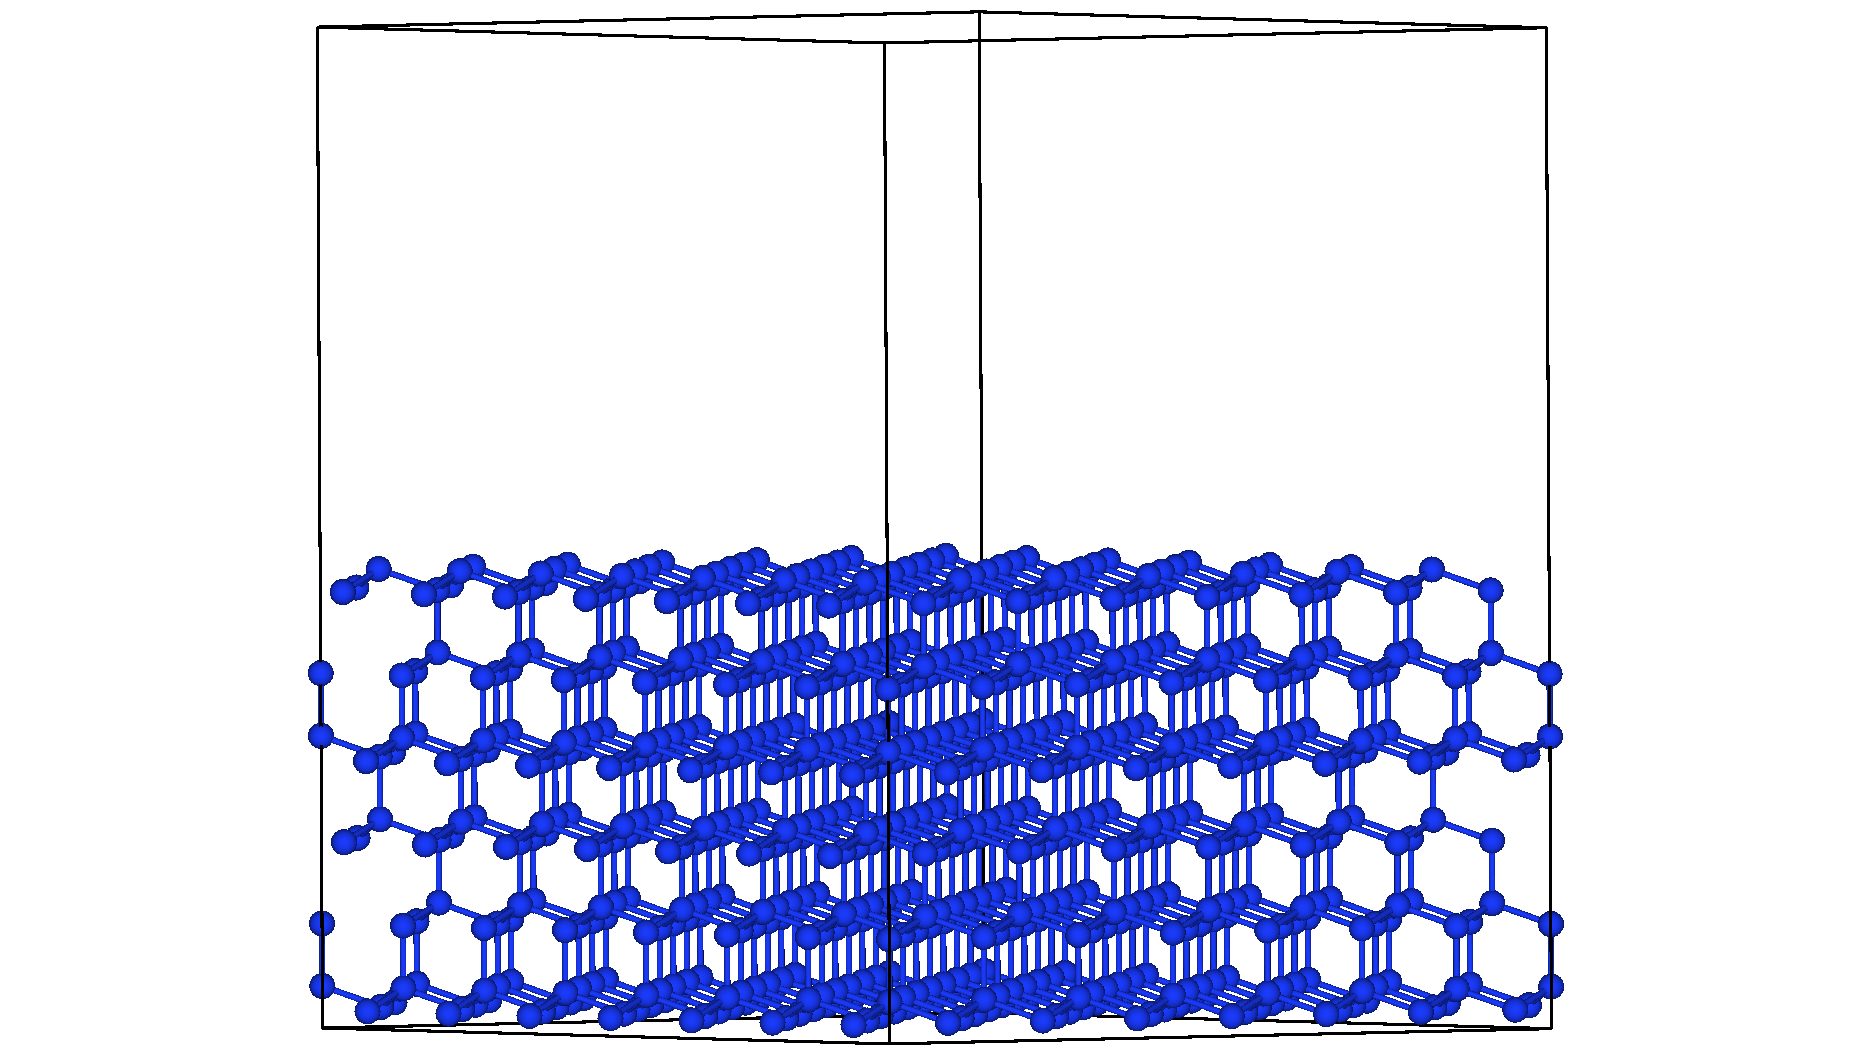
\includegraphics[width=\textwidth]{Si_surf.png} 
   \caption{Si(111) surface supercell with a $7\times7$ primitive cells in the $ab$ plane.}
   \label{surfSi}
\end{figure}



\newpage
\appendix
\section{Technicalities}\label{techappendix}

\subsection{Order in which things are done in the supercell generation}
Note the order, and in particular the units in which the operations are done. The 
\begin{enumerate}
\item Generation of primitive cell (or the conventional cell, if the flag \texttt{--no-reduce} is used).
\item Rotation/rescaling transformation of the lattice vectors with \texttt{--transform-cell}.
\item Applying supercell map with \texttt{--supercell=\ldots}. The units are the previously generated primitive or conventional cell.
\item Moving atoms in the supercell by \texttt{--supercell-translation-vector} \emph{or} \\ \texttt{--supercell-prevacuum-translation} (in units of the supercell!).
\item Adding vacuum along the direction of one of the lattice vectors with \texttt{--supercell-vacuum} (in units of the supercell!).
\item Moving atoms in the supercell by \texttt{--supercell-postvacuum-translation} (in units of the supercell including vacuum!).
\end{enumerate}

%\newpage
%\begin{landscape}
\begin{table}[htdp]
\caption{Various useful transformations. Spotting the system in the three last ones, we see that you get successively larger hexagonal surface cells by just adding 1 to the two upper left diagonal elements. The "square root sequence" begins $\sqrt{3}$, $\sqrt{7}$, $\sqrt{13}$, $\sqrt{21}$, $\sqrt{31}$, $\sqrt{43}$\ldots}
\begin{center}
\begin{tabular}{c|c|c}
Transform this\ldots & \ldots into that\ldots & \ldots with this \\\hline\hline
%\T Standard fcc & fcc lattice vectors in & \\
%lattice vectors & standard rhombohedral setting& \\
%$\begin{pmatrix}
%\frac{1}{2} & \frac{1}{2} & 0 \\
%\frac{1}{2} & 0 & \frac{1}{2} \\
%0 & \frac{1}{2} & \frac{1}{2}
%\end{pmatrix}$ & 
%$\begin{pmatrix}
%\frac{1}{\sqrt{3}} & 0 & \sqrt{\frac{2}{3}} \\
%-\frac{1}{\sqrt{12}} & \frac{1}{2} & \sqrt{\frac{2}{3}} \\
%-\frac{1}{\sqrt{12}} & -\frac{1}{2} & \sqrt{\frac{2}{3}}
%\end{pmatrix}$ & 
%$\begin{pmatrix}
%\frac{1-\sqrt{2}}{\sqrt{3}} & \frac{1+\sqrt{2}}{\sqrt{3}} & \frac{\sqrt{2}-1}{\sqrt{3}} \\
%\frac{\sqrt{3}-1-2\sqrt{2}}{\sqrt{12}} & \frac{-\sqrt{3}-1+2\sqrt{2}}{\sqrt{12}} & 1- \frac{\sqrt{3}-1-2\sqrt{2}}{\sqrt{12}} \\
%-1+\frac{\sqrt{3}-1-2\sqrt{2}}{\sqrt{12}}  & 1+\frac{-\sqrt{3}-1+2\sqrt{2}}{\sqrt{12}} & \frac{1-\sqrt{3}+2\sqrt{2}}{\sqrt{12}}
%\end{pmatrix}$ \BM \\\hline
\T Standard rhombohedral & Standard hexagonal & \multirow{3}{*}{$\begin{pmatrix} 1& -1 & 0\\0 & 1& -1\\ 1&1 &1 \end{pmatrix}$}\\
cell with threefold axis & cell with sixfold axis & \\
along the $z$ direction & along the $z$ direction & \B \\\hline
\TM $\begin{pmatrix}
\frac{1}{2} & \frac{1}{2} & 0 \\
\frac{1}{2} & 0 & \frac{1}{2} \\
0 & \frac{1}{2} & \frac{1}{2}
\end{pmatrix}$ &
$\begin{pmatrix}
1 & 0 & 0\\
0 & 1 & 0\\
0 & 0 & 1
\end{pmatrix}$ &
$\begin{pmatrix}
1 & 1 & -1\\
1 & -1 & 1\\
-1 & 1 & 1
\end{pmatrix}$\BM \\\hline
\TM $\begin{pmatrix}
-\frac{1}{2} & \frac{1}{2} & \frac{1}{2} \\
\frac{1}{2} & -\frac{1}{2} & \frac{1}{2} \\
\frac{1}{2} & \frac{1}{2} & -\frac{1}{2}
\end{pmatrix}$ &
$\begin{pmatrix}
1 & 0 & 0\\
0 & 1 & 0\\
0 & 0 & 1
\end{pmatrix}$ &
$\begin{pmatrix}
0 & 1 &  1\\
1 &  0 & 1\\
1 & 1 & 0
\end{pmatrix}$ \BM \\\hline
\T & $(\sqrt{3}\times\sqrt{3})R30^{\circ}$ & \multirow{3}{*}{$\begin{pmatrix} 2 &  1 & 0\\-1 & 1&  0\\ 0&0 &1 \end{pmatrix}$}\\
Hexagonal unit cell & hexagonal cell & \\
& & \\\hline
\T & $(\sqrt{7}\times\sqrt{7})R19^{\circ}$ & \multirow{3}{*}{$\begin{pmatrix} 3 &  1 & 0\\-1 & 2&  0\\ 0&0 &1 \end{pmatrix}$}\\
Hexagonal unit cell & hexagonal cell & \\
& & \\\hline
\T & $(\sqrt{13}\times\sqrt{13})R??^{\circ}$ & \multirow{3}{*}{$\begin{pmatrix} 4 &  1 & 0\\-1 & 3&  0\\ 0&0 &1 \end{pmatrix}$}\\
Hexagonal unit cell & hexagonal cell & 
\end{tabular}
\end{center}
\label{transformations}
\end{table}%

%\end{landscape}


\end{document}  